\section{Derivation of Actuator Model}

\begin{figure}[t]
\centering
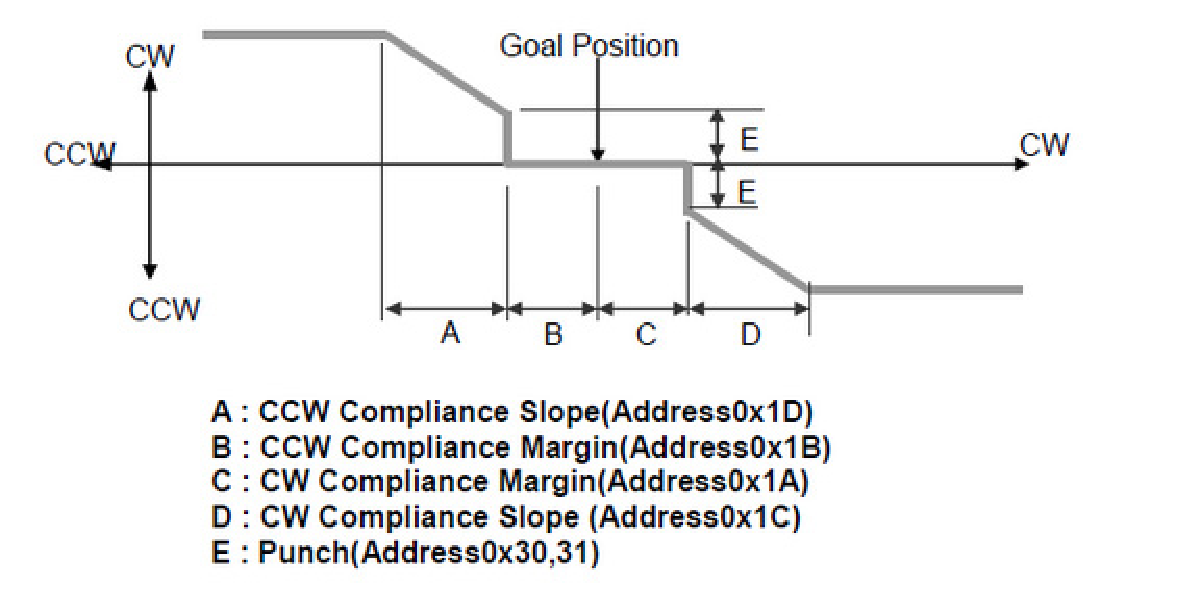
\includegraphics[width=0.45\textwidth]{figures/ax18gain.eps}
\caption{The mapping between $q-\bar{q}$ and $U$ for an AX-18 actuator \cite{AX18:2015}. The x-axis is $q-\bar{q}$ while the y-axis is $U$.}
\vspace{-0.1in}
\label{fig:actuatorMap}
\end{figure}

In this Appendix, we derive the actuator model (eq.(\ref{eqn:torqueErrorRelationSimple})) from the specifications of the Dynamixel AX-18 servo (Figure \ref{fig:actuatorMap}). The servo maps the difference between the desired and the actual joint angle $q-\bar{q}$ to the power level $U$. The intervals A and D determine the proportion gain for counter-clockwise and clockwise motions respectively. B and C are the compliance margins, which are thresholds below which the servo stops outputting any torque. E, the punch, is the minimum power level before the servo shuts down. In practice, we set A and D the same. In addition, since B, C and E are much smaller than A or D, we ignore their effects and approximate the mapping as linear within the intervals $q-\bar{q}\in A\bigcup B\bigcup C\bigcup D$ with the slope $k_e$:
\begin{displaymath}
  U=k_e(q-\bar{q})
\end{displaymath}

To derive the relation between the power level $U$ and the output torque $\tau$, we adopt a model for the ideal DC motor \cite{SchwarzB:2013}. It is a valid assumption because the AX-18 servos use high-quality DC motors. Considering the power balance in the motor at a constant voltage U:
\begin{equation}
  P_{electric} = P_{mechanic} + P_{heat}
  \label{eqn:powerBalance}
\end{equation}
The electrical power $P_{electric}$ can be decomposed into the mechanical power $P_{mechanic}$ and the heat $P_{heat}$. From eq.(\ref{eqn:powerBalance}), we can get the following relation:
\begin{equation}
UI=\dot{q}\tau_{motor} + RI^2
\end{equation}
where $I$ is the current and $R$ is the motor winding resistance. In an ideal DC motor, the torque is linearly proportional to the current $\tau_{motor}=k_{\tau}I$. Plugging it into the above equation, we have:
\begin{equation}
  U=k_{\tau}\dot{q}+\frac{R}{k_{\tau}}\tau_{motor}
  \label{eqn:votageTorqueRelation}
\end{equation}
where $k_{\tau}$ is the torque constant. The total torque $\tau_{motor}$ is the sum of the output torque $\tau$ that drives the motor shaft and the frictional torque $\tau_f$ inside the motor:
\begin{equation}
  \tau_{motor}=\tau+\tau_f
  \label{eqn:torqueBalance}
\end{equation}
The friction torque can be further divided into viscous friction and Coulomb friction \cite{SchwarzB:2013}:
\begin{equation}
  \tau_f = k_v\dot{q}+k_c\sgn(\dot{q})
  \label{eqn:frictionComponents}
\end{equation}
where $k_v$ and $k_c$ are friction coefficients for the viscous and Coulomb friction respectively. $\sgn(x)$ is the sign function that equals 1 if $x$ is positive, -1 if $x$ is negative and 0 otherwise.

Combining eq.(\ref{eqn:votageTorqueRelation}), (\ref{eqn:torqueBalance}) and (\ref{eqn:frictionComponents}), we get the actuator model (eq.(\ref{eqn:torqueErrorRelationSimple})):
\begin{align}
\nonumber  \tau & = \frac{k_{\tau}k_e}{R}(q-\bar{q})+(-k_v-\frac{k_{\tau}^2}{R})\dot{q}-k_c\sgn(\dot{q})\\
\nonumber & = -k_p(q-\bar{q}) - k_d\dot{q} - k_c\sgn(\dot{q})
\end{align}
where $k_p=-\frac{k_{\tau}k_e}{R}$ and $k_d=k_v+\frac{k_{\tau}^2}{R}$. 
